\documentclass[10pt,a4paper]{article}
\usepackage[utf8x]{inputenc}
\usepackage{ucs}
\usepackage[left=2.00cm, right=2.00cm, top=2.00cm, bottom=2.00cm]{geometry}
\renewcommand\familydefault{\sfdefault}

\title{Summary - \lecture}
\author{}
\date{}


%costum layout
\setlength{\parindent}{0cm}
\usepackage{fancyhdr}
\pagestyle{fancy}
\fancyhf{}
\fancyhead[L]{
	\strut\rlap{\colorlayout\rule[-\dp\strutbox]{\headwidth}{\headheight}}
	\textcolor {white} {Summary: \lecture}}
\fancyfoot[L]{
	\strut\rlap{\colorlayout\rule[-\dp\strutbox]{\headwidth}{\headheight}}
	\textcolor {white} {last changed: \today}}
\fancyhead[R]{\textcolor{white}{\semseter}}
\fancyfoot[R]{\textcolor{white} {\thepage}}


%math
\usepackage{amsmath}
\usepackage{amsfonts}
\usepackage{amssymb}
\usepackage{amstext}
\usepackage{mathtools}


%graphics
\usepackage{graphicx}
\usepackage{floatflt}
\usepackage{float}


%tabular
\usepackage{tabularx}
\usepackage[font=small,labelfont=small]{caption}
\usepackage{colortbl}
\usepackage[dvipsnames]{xcolor}
\renewcommand{\arraystretch}{1}
%\arrayrulecolor{white}


%tikz
\usepackage{tikz}
\usetikzlibrary{shapes, petri}
\tikzstyle{ell}=[ellipse,draw, yshift=-2mm]
\tikzstyle{rec} = [rectangle, draw]
\tikzstyle{dia} = [diamond, aspect=2, draw, yshift=-5mm]
\tikzstyle{cir} = [circle, draw, minimum size=3mm]
\tikzstyle{arrHV} = [to path={-| (\tikztotarget)}]
\tikzstyle{arrVH} = [to path={|- (\tikztotarget)}]
\tikzstyle{whileright} = [xshift=20mm, yshift=-3mm]
\tikzstyle{whileleft} = [xshift=-20mm, yshift=-3mm]
\tikzstyle{txtright} = [above, xshift=15mm]
\tikzstyle{txtleft} = [above, xshift=-15mm]
\tikzstyle{empty} = [coordinate]
\usetikzlibrary{positioning}


%listings
\usepackage{listings}
\lstdefinestyle{costum} {
	language=Bash,
	basicstyle=\footnotesize\ttfamily,
	keywordstyle=\bfseries\color{cyan!50!blue},
	commentstyle=\itshape\color{black!50},
	%identifierstyle=\color{blue},
	stringstyle=\color{green!50!black},
	morekeywords={returns, loop, each},
	escapeinside={\%*}{*)}
}
\lstset{style=costum}


%custom title color
\usepackage{titlesec}
\setcounter{secnumdepth}{4}

\titleformat{\section}
{\color{cyan!80!blue}\normalfont\Large\bfseries}
{\color{cyan!80!blue}\thesection}{1em}{}

%\titleformat{\subsubsection}
%{\color{blue!30!black!70}\normalfont\bfseries}
%{\color{black}\thesection}{1em}{}
%
%\titleformat{\paragraph}
%{\color{green!30!black!70}\normalfont\normalsize\bfseries}{\theparagraph}{1em}{}
%\titlespacing*{\paragraph}
%{0pt}{3.25ex plus 1ex minus .2ex}{1.5ex plus .2ex}


%tab
\newcommand{\tab}[1][1]{\hspace*{#1cm}}


%hyperref
\usepackage{hyperref}


%vector
\newcommand{\vect}[1]{\ensuremath{\begin{bmatrix}#1\end{bmatrix}}}

\usepackage{pgfplots}

%TODO
%config
\newcommand{\lecture}{Introduction to Deep Learning} %title of the lecture
\newcommand{\lecturer}{Nießner M.} %lecturer of the lecture
\newcommand{\semseter}{summer semester 2020} %semester of this lecture, e.g., summer semester 2019
\newcommand{\colorlayout}{\color{cyan!50!blue}} %color of the title bar, see colors

%colors, e.g,
%cyan!50!blue
%green!50!black
%orange!50!black

%user
\newcommand{\cons}{\textcolor{red}{\textbf{-}}}
\newcommand{\pros}{\textcolor{green}{\textbf{+}}}


%TODO
% a user defined todo list



\begin{document}
\tableofcontents
\pagebreak

\section{Machine Learning Basics}
\subsection{Un-/Supervised Learning}
\begin{itemize}
	\item Unsupervised Learning
	\begin{itemize}
		\item No label or target class
		\item Find out properties of the structure of the data
		\item clustering (k-means, PCA, etc.)
	\end{itemize}
	\item Supervised Learning
	\begin{itemize}
		\item Labels or target classes
	\end{itemize}
	\item Reinforcement Learning
\end{itemize}

\pagebreak
\section{Linear Models}
\subsection{Regression, Classification}
\begin{itemize}
	\item \textbf{Regression:} Predicts a continuous output value
	\item \textbf{Classification:} Predicts a discrete value
	\begin{itemize}
		\item \textbf{Binary Classification:} Output either $0$ or $1$
		\item \textbf{Multi-class classification:} Set of N classes
	\end{itemize}
\end{itemize}

\subsection{Obtaining the model}
\begin{enumerate}
	\item Estimating using current model
	\item Calculating loss
	\item Optimizing the model
\end{enumerate}

\subsection{Linear Regression}
\subsubsection{Linear Model}
\begin{tabular}{ll}
	$i$: & index of current sample \\
	$j$: & index of current weight \\
	$d$: & input dimension/number of weights \\
	$x_{ij}$: & $i$-th input data/feature of the $j$-th weight \\
	$\theta_0$: & bias \\
	$\theta_j$: & weights \\
	$\hat y_i$: & $i$-th Prediction/Estimation (predicted label)
\end{tabular}

$$
	\hat y_i = \theta_0 + \sum_{j = 1}^d x_{ij} \theta_j = \theta_0 + x_{i1} \theta_1 + \dots + x_{id} \theta_d
$$

\textbf{Matrix Notation:}
$$
	\hat y = X \theta
$$

\subsubsection{Loss function}
Measures how good my estimation is and tells the optimization method how to make it better

\paragraph{Linear Least Squares:} ~\\
\begin{tabular}{ll}
	$n$: & number of training samples \\
	$y$: & Ground truth labels \\
	$\hat y$: & Estimated labels
\end{tabular}
$$
	J(\theta) = \frac 1 n \sum_{i = 1}^n (\hat y_i - y_i)^2
$$

\textbf{Matrix Notation:}
$$
	J(\theta) = (X \theta - y)^T (X \theta - y) = (\hat y - y)^T (\hat y - y)
$$

\subsubsection{Optimization}
Changes the model in order to improve the loss function/estimation
$$
	\theta = (X^TX)^{-1}X^Ty
$$

\subsection{Logistic Regression}
\subsubsection{Model}
\begin{tabular}{ll}
	$i$: & index of current sample \\
	$j$: & index of current weight \\
	$d$: & input dimension/number of weights \\
	$x_{ij}$: & $i$-th input data/feature of the $j$-th weight \\
	$\theta_j$: & model parameters \\
	$\hat y_i$: & $i$-th Prediction/Estimation (predicted label)
\end{tabular}

$$
	\hat y_i = \sigma(x_i \theta) = \sigma \left(\sum_{j = 1}^d x_{ij} \theta_j \right)
$$
with
$$
	\sigma(x) = \frac 1 {1 + e^{-x}}
$$

\subsubsection{Loss function}
Measures how good my estimation is and tells the optimization method how to make it better

\paragraph{Binary Cross-Entropy:} ~\\
\begin{tabular}{ll}
	$y$: & Ground truth labels \\
	$\hat y$: & Estimated labels
\end{tabular}
$$
	\mathcal L(\hat y_i, y_i) = y_i \log \hat y_i + (1 - y_i) \log (1 - \hat y_i)
$$

\subsubsection{Cost function}
\begin{tabular}{ll}
	$n$: & number of labels
\end{tabular}
$$
	C(\theta) = - \frac 1 n \sum_{i = 1}^n \mathcal L(\hat y_i, y_i)
$$

\subsubsection{Optimization}
Changes the model in order to improve the loss function/estimation
\begin{itemize}
	\item No closed-form solution
	\item Make use of an iterative method e.g. Gradient Descent
\end{itemize}

\section{Computational Graphs}
\begin{itemize}
	\item Directional graph
	\item Matrix operations are represented as compute graphs
	\item Vertex nodes are variables or operators like $+, -, *, /, log(), exp(), \dots$
	\item Directional edges show flow of inputs to vertices
	\item Neural network can be represented as computational graph
\end{itemize}

\subsection{Graphical representation}
\textbf{Example}
$$
	f(x, y, z) = (x + y) ⋅ z
$$
\begin{figure}[H]
	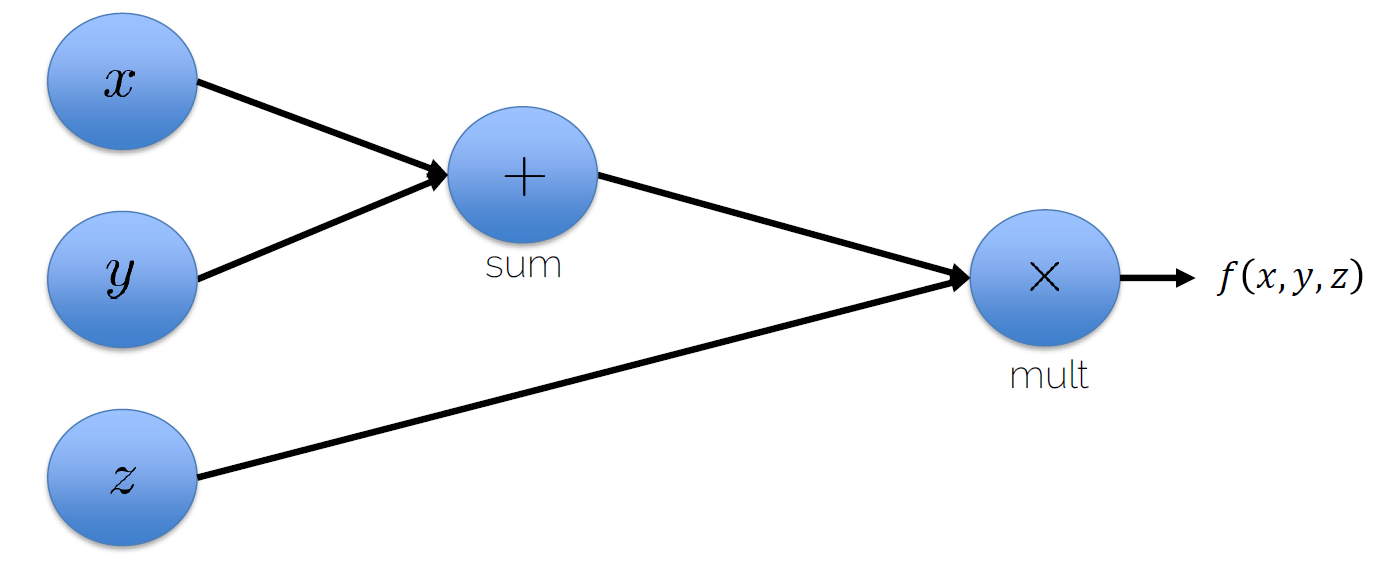
\includegraphics[width=\columnwidth]{figures/comp_graph.png}
\end{figure}

\textbf{Neural Network as Computational Graph}
\begin{figure}[H]
	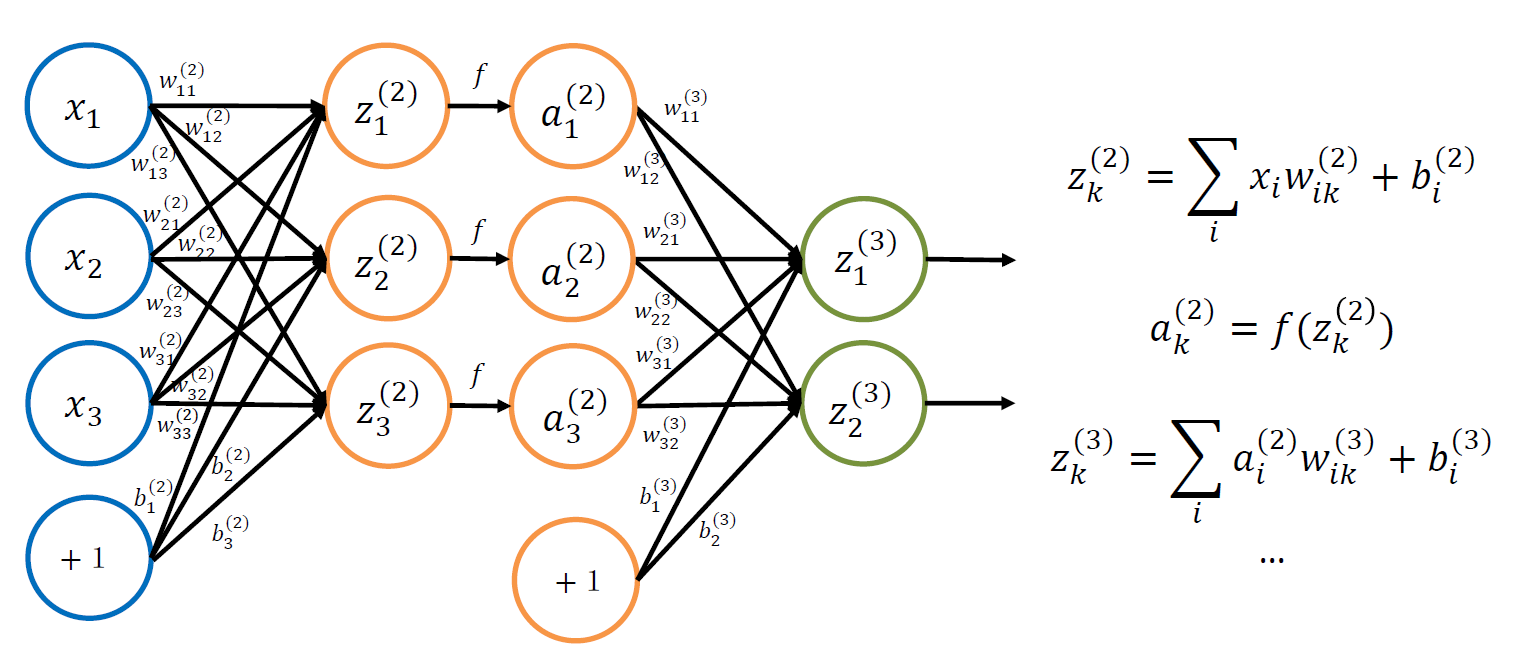
\includegraphics[width=\columnwidth]{figures/comp_graph_nn.png}
\end{figure}

\section{Neural Network}
\subsection{Activation Functions}
\textbf{Description} \\
%TODO

\textbf{Parameters:} \\
\begin{tabular}{ll}
	$\hat y$: & Prediction \\
	$\hat y_j$: & Prediction of $j$-th output ($j$-th Neuron of output layer) \\
	$h$: & Outputs of hidden layer \\
	$s$: & Output of layer (before activation) \\
	$s_j$: & Output of the $j$-th neuron in layer (before activation) \\
	$C$: & Number of classes (number of neurons in output layer)
\end{tabular}

\subsubsection{Sigmoid}
\begin{itemize}
	\item Used for Binary Classification to output a probability matching first or second class
	\item \textbf{Output:} $\hat y = (0, 1)$
	\item If used as activation function in hidden layer (typically it is not)
	\begin{itemize}
		\item[\cons] Output is always positive
		\item[\cons] Saturates for high positive or low negative values → kills the gradient flow
	\end{itemize}	
\end{itemize}
\begin{tabularx}{\columnwidth}{XX}
	$$
	\sigma(s) = \frac 1 {1 + e^{-s}}
	$$ &\\&
	
	\begin{tikzpicture}
	\begin{axis}[
	xmin=-10, xmax=10,
	ymin=-0, ymax=1,
	axis y line=middle,
	axis x line=middle,
	]
	\addplot+[domain=-10:10, samples=100, mark=none] {1/(1 + exp(-x))};
	\end{axis}
	\end{tikzpicture}
\end{tabularx}

\subsubsection{Softmax}
\begin{itemize}
	\item Used for Multiclass Classification to output a probability matching the $i$-th class
	\item \textbf{Output:} $\hat y_j = (0, 1)$
\end{itemize}

$$
	\hat y_j = \frac{e^{s_j}}{\sum_{k = 1, k ≠ j}^{C} e^{s_k}}
$$


\subsubsection{Tanh (Hyperbolic Tanjant Function)}
\begin{itemize}
	\item[\cons] Saturates for high positive or low negative values → kills the gradient flow
\end{itemize}

\begin{tabularx}{\columnwidth}{XX}	
	$$
		h = \tanh(s)
	$$ &\\&
	
	\begin{tikzpicture}
	\begin{axis}[
	xmin=-10, xmax=10,
	ymin=-1, ymax=1,
	axis y line=middle,
	axis x line=middle,
	]
	\addplot+[domain=-10:10, samples=100, mark=none] {tanh(x)};
	\end{axis}
	\end{tikzpicture}
\end{tabularx}

\subsubsection{ReLU (Rectified Linear Units)}
\begin{itemize}
	\item Standard choice for activation function
	\item[\pros] Does not saturate
	\item[\pros] Large and consistent gradients
	\item[\pros] Fast convergence
	\item[\cons] Dead ReLU if output is zero
	\item Initialization of ReLU neurons with slightly positive biases (e.g. $0.01$) → Likely to stay active for most inputs
\end{itemize}

\begin{tabularx}{\columnwidth}{XX}	
	$$
		h = \max(0, s)
	$$ &\\&
	
	\begin{tikzpicture}
	\begin{axis}[
	xmin=-10, xmax=10,
	ymin=0, ymax=10,
	axis y line=middle,
	axis x line=middle,
	]
	\addplot+[domain=-10:10, samples=100, mark=none] {max(0,x)};
	\end{axis}
	\end{tikzpicture}
\end{tabularx}

\subsubsection{Leaky ReLU}
\begin{itemize}
	\item[\pros] Does not die
\end{itemize}

\begin{tabularx}{\columnwidth}{XX}	
	$$
		h = \max(0.1s, s)
	$$ &\\&
	
	\begin{tikzpicture}
	\begin{axis}[
	xmin=-10, xmax=10,
	ymin=-1, ymax=10,
	axis y line=middle,
	axis x line=middle,
	]
	\addplot+[domain=-10:10, samples=100, mark=none] {max(0.1*x,x)};
	\end{axis}
	\end{tikzpicture}
\end{tabularx}

\subsubsection{Parametric ReLU}
\begin{itemize}
	\item[\pros] Does not die
\end{itemize}

$$
	h = \max(\alpha s, s)
$$

\subsubsection{ELU}
$$
f(s) = \begin{cases}
s & \text{if } s > 0 \\
\alpha (e^s - 1) & \text{if } s ≤ 0
\end{cases}
$$

\subsubsection{Maxout}
\begin{itemize}
	\item[\pros] Generalization of ReLUs
	\item[\pros] Linear regimes
	\item[\pros] Does not die
	\item[\pros] Does not saturate
	\item[\cons] Increases the number of parameters
\end{itemize}
$$
 	h = \max(w_1^Ts + b_1, w_2^T s + b_2)
$$

\subsubsection{Step Function}
\begin{tabularx}{\columnwidth}{XX}	
	$$
		h = \begin{cases}
			0 & \text{if } s < 0 \\
			1 & \text{if } s ≥ 0 \\
		\end{cases}
	$$ &\\&
	
	\begin{tikzpicture}
	\begin{axis}[
	xmin=-10, xmax=10,
	ymin=-1, ymax=2,
	axis y line=middle,
	axis x line=middle,
	]
	\addplot+[blue, domain=-10:0, samples=100, mark=none] {0};
	\addplot+[blue, domain=0:10, samples=100, mark=none] {1};
	\end{axis}
	\end{tikzpicture}
\end{tabularx}


\subsection{Loss Function}
\subsubsection{Description}
A function to measure the goodness of the predictions
\begin{itemize}
	\item Large loss $\implies$ bad predictions
	\item Goal: Minimize the loss $\iff$ Find better predictions
	\item Choice of the loss function depends on the concrete problem or the distribution of the target variable
\end{itemize}

\subsubsection{Parameters}
\begin{tabular}{ll}
	$y_i$: & Ground truth of $i$-th sample \\
	$\hat y_i$: & Prediction of $i$-th sample \\
	$n$: & number of training samples \\
	$k$: & number of classes \\
	$\hat y_{i, gt}$: & Prediction of ground truth class of $i$-th sample (where $y_{ij} = 1$)
\end{tabular}

\subsubsection{L1 Loss}
\begin{itemize}
	\item Sum of absolute differences
	\item Robust (cost of outliers is linear)
	\item Costly to optimize
	\item Optimum is median
\end{itemize}
$$
	\mathcal L(y, \hat y; \theta) = \frac 1 n \sum_i^n ||y_i - \hat y_i||_1
$$

\subsubsection{L2/MSE Loss}
\begin{itemize}
	\item Sum of squared differences
	\item Prone to outliers
	\item Compute-efficient optimization
	\item Optimum is mean
\end{itemize}
$$
	\mathcal L(y, \hat y; \theta) = \frac 1 n \sum_i^n ||y_i - \hat y_i||_2^2
$$

\subsubsection{Binary Cross Entropy}
$$
	\mathcal L(y, \hat y; \theta) = - \frac 1 n \sum_{i = 1}^n (y_i \log \hat y_i + (1 - y_i) \log(1 - \hat y_i))
$$

\subsubsection{Cross Entropy}
\begin{itemize}
	\item Loss is typically always $> 0$ → Always improvement
\end{itemize}
$$
	\mathcal L(y, \hat y; \theta) = - \frac 1 n \sum_{i = 1}^n \sum_{j = 1}^k (y_{ij} \log \hat y_{ij})
$$

\subsubsection{Hinge Loss (SVM Loss)}
\begin{itemize}
	\item Loss can become $= 0$ → Saturation
\end{itemize}
$$
	\mathcal L(y, \hat y; \theta) = \frac 1 n \sum_{i = 1}^n \sum_{{j = 1,} \atop {j ≠ gt}}^k \max(0, \hat y_{ij} - \hat y_{i,gt} + 1)
$$


\subsection{Optimization Functions}
\subsubsection{General Optimization}
\begin{itemize}
	\item \textbf{Goal:} $\theta^* = \arg\min f(\theta, x, y)$
	\item \textbf{Linear Systems (Ax = b)}
	\begin{itemize}
		\item LU, QU, Cholesky, Jacobi, Gauss-Seidel, CG, PCG, ...
	\end{itemize}
	\item \textbf{Non-linear systems} (Gradient based methods):
	\begin{itemize}
		\item First order methods:
		\begin{itemize}
			\item Gradient Descent, SGD, SGD with Momemtum, RMSProp, Adam (Standard)
		\end{itemize}
		\item Second order methods (faster than first order methods, but only for full batch updates):
		\begin{itemize}
			\item Newton, Gauss-Newton, Levenberg-Marquardt, (L)BFGS
		\end{itemize}
	\end{itemize}
\end{itemize}


\subsubsection{Gradient Descent}
\begin{itemize}
	\item Finds local minimum
	\item Does not guarantee to find global optimum
	\item Does gradient steps in direction of negative gradient
	\item[\cons] Requires a lot of memory $\implies$ extremely expensive
\end{itemize}

Parameters: \\
\begin{tabular}{ll}
	$f(\theta, x_{1..n}, y_{1..n})$: & Function describing the neural network (including loss function) \\
	$x_{1..n}$: & Input vectors for all $n$ training samples \\
	$y_{1..n}$: & Ground truth for all $n$ training samples \\
	$\theta^k = \{W, b\}$: & Model Parameters at step $k$ \\
	$\alpha$: & Learning rate
\end{tabular} \\

Gradient Step:
$$
	\theta^{k + 1} = \theta^k - \alpha \nabla_\theta f(\theta^k, x_{1..n}, y_{1..n})
$$

\subsubsection{Stochastic Gradient Descent}
\begin{itemize}
	\item Split training set into several minibatches
	\item Minibatch size:
	\begin{itemize}
		\item Is a hyperparameter
		\item Is typically a power of 2
		\item Smaller batch size $\implies$ Greater variance in the gradients
		\item Is mostly limited by GPU memory
	\end{itemize}
	\item Epoch: Complete pass through training set
	\item[\cons] Cannot independently scale directions
	\item[\cons] Need to have conservative min learning rate to avoid divergence
	\item[\cons] Is slower than necessary
\end{itemize}

Parameters: \\
\begin{tabular}{ll}
	$n$: & Number of total training samples \\
	$m$: & Minibatch size (number of training samples per minibatch) \\
	$n/m$: & Number of minibatches \\
	$f(\theta, x_{1..m}, y_{1..m})$: & Function describing the neural network (including loss function) \\
	$x_{1..m}$: & Input vectors for one minibatch \\
	$y_{1..m}$: & Ground truth for one minibatch \\
	$\theta^k = \{W, b\}$: & Model Parameters at step $k$\\
	$k$: & iteration in current epoch \\
	$\alpha$: & Learning rate
\end{tabular} \\

Gradient Step:
$$
	\theta^{k + 1} = \theta^k - \alpha \nabla_\theta f(\theta^k, x_{1..m}, y_{1..m})
$$

\paragraph{Convergence of Stochastic Gradient Descent} ~\\
$f(\theta, x, y)$ converges to a local (global) minimum if:
\begin{enumerate}
	\item $\alpha_n ≥ 0, \forall n ≥ 0$
	\item $\sum_{n = 1}^∞ \alpha_n = ∞$
	\item $\sum_{n = 1}^∞ \alpha_n^2 < ∞$
	\item $f(\theta, x, y)$ ist strictly convex
\end{enumerate}
where $\alpha_1, \dots, \alpha_n$ is a sequence of positive step-sizes

\subsubsection{Gradient Descent with Momentum}
\begin{itemize}
	\item Step will be largest when a sequence of gradients all point to the same direction
\end{itemize}

Parameters: \\
\begin{tabular}{ll}
	$f(\theta, x, y)$: & Function describing the neural network (including loss function) \\
	$x$: & Input vectors \\
	$y$: & Ground truth \\
	$\theta^k = \{W, b\}$: & Model Parameters at step $k$\\
	$\alpha$: & Learning rate \\
	$\beta$: & Accumulation rate (friction, momentum), default: 0.9 \\
	$v^k$: & velocity at step $k$ \\
\end{tabular} \\

Gradient step:
$$
	v^{k + 1} = \beta ⋅ v^k - \alpha ⋅ \nabla_\theta f(\theta^k, x, y)
$$
$$
	\theta^{k + 1} = \theta^k + v^{k + 1}
$$

\subsubsection{Nesterov Momentum}
\begin{itemize}
	\item Look-ahead momentum
	\item Steps:
	\begin{enumerate}
		\item Make a big jump in the direction of the previous accumulated gradient
		\item Measure the gradient where you end up
		\item Make a correction
	\end{enumerate}
\end{itemize}

Parameters: \\
\begin{tabular}{ll}
	$f(\theta, x, y)$: & Function describing the neural network (including loss function) \\
	$x$: & Input vectors \\
	$y$: & Ground truth \\
	$\theta^k = \{W, b\}$: & Model Parameters at step $k$\\
	$\alpha$: & Learning rate \\
	$\beta$: & Accumulation rate (friction, momentum), default: 0.9 \\
	$v^k$: & velocity at step $k$ \\
\end{tabular} \\

Gradient step:
$$
	\tilde \theta^{k + 1} = \theta^k + \beta ⋅ v^k
$$
$$
	v^{k + 1} = \beta ⋅ v^k - \alpha ⋅ \nabla_\theta f(\tilde \theta^{k + 1}, x, y)
$$
$$
	\theta^{k + 1} = \theta^k + v^{k + 1}
$$

\subsubsection{Root Mean Squared Prop (RMSProp)}
\begin{itemize}
	\item Divides the learning rate by an exponentially-decaying average of squared gradients
	\item Damps the oscillations for high-variance directions
	\item[\pros] Can increase learning rate because it is less likely to diverge → Speeds up learning speed
\end{itemize}

Parameters: \\
\begin{tabular}{ll}
	$f(\theta, x, y)$: & Function describing the neural network (including loss function) \\
	$x$: & Input vectors \\
	$y$: & Ground truth \\
	$\theta^k = \{W, b\}$: & Model Parameters at step $k$\\
	$\alpha$: & Learning rate \\
	$\beta$: & Accumulation rate (friction, momentum), default: $0.9$ \\
	$\epsilon$: & Prevents division by zero, default: $10^{-8}$ \\
	$s^k$: & Second momentum (uncentered variance of gradients)
\end{tabular} \\

Gradient step:
$$
	s^{k + 1} = \beta ⋅ s^k + (1 - \beta)(\nabla_\theta f(\theta^k, x, y) \circ \nabla_\theta f(\theta^k, x, y))
$$
$$
	\theta^{k + 1} = \theta^k - \alpha ⋅ \frac{\nabla_\theta f(\theta^k, x, y)}{\sqrt{s^{k + 1}} + \epsilon}
$$
where $a \circ b$ is an element-wise multiplication

\subsubsection{Adaptive Momemt Esimation (Adam)}
\begin{itemize}
	\item Combines Momentum and RMSProp
	\item Combines first and second order momentum
\end{itemize}

Parameters: \\
\begin{tabular}{ll}
	$f(\theta, x, y)$: & Function describing the neural network (including loss function) \\
	$x$: & Input vectors \\
	$y$: & Ground truth \\
	$\theta^k = \{W, b\}$: & Model Parameters at step $k$\\
	$\alpha$: & Learning rate \\
	$\beta_1$: & Accumulation rate 1, default: $0.9$ \\
	$\beta_2$: & Accumulation rate 2, default: $0.999$ \\
	$\epsilon$: & Prevents division by zero, default: $10^{-8}$ \\
	$s^k$: & Second momentum (uncentered variance of gradients)
\end{tabular} \\

Gradient step:
$$
	\hat m^{k + 1} = \frac{\beta_1 ⋅ m^k + (1 -\beta_1) ⋅ \nabla_\theta f(\theta^k, x, y)}{1 - \beta_1^{k + 1}}
$$
$$
	\hat v^{k + 1} = \frac{\beta_2 ⋅ v^k + (1 - \beta_2)(\nabla_\theta f(\theta^k, x, y) \circ \nabla_\theta f(\theta^k, x, y))}{1 - \beta_2^{k + 1}}
$$
$$
	\theta^{k + 1} = \theta^k - \alpha ⋅ \frac{\hat m^{k + 1}}{\sqrt{\hat v^{k + 1}} + \epsilon}
$$
where $m^0 = v^0 = 0$

\subsubsection{Newton's Method}
\begin{itemize}
	\item Computation complexity of inversion per iteration: $\mathcal O(k^3)$
\end{itemize}

Parameters: \\
\begin{tabular}{ll}
	$f(\theta)$: & Function describing the neural network (including loss function) \\
	$\theta = \{W, b\}$: & Model Parameters \\
	$\nabla_\theta f(\theta)$: & Gradient (first derivative) \\
	$H(\theta)$: & Hessian matrix (second derivative)
\end{tabular} \\

Approximate the function by a second-order Taylor series expansion
$$
	f(\theta) \approx f(\theta_0) + (\theta - \theta_0)^T \nabla_\theta f(\theta_0) + \frac 1 2 (\theta - \theta_0)^T H(\theta - \theta_0)
$$

Update step:
$$
	\theta^* = \theta_0 - H^{-1} \nabla_\theta f(\theta)
$$

\subsubsection{Broyden-Fletcher-Goldfarb-Shanno algorithm (BFGS and L-BFGS)}
\begin{itemize}
	\item Belongs to the family of quasi-Newton methods
	\item Have an approximation of the inverse of the Hessian
	\item Computation complexity of inversion per iteration:
	\begin{itemize}
		\item BFGS: $\mathcal O(n^2)$
		\item L-BFGS: $\mathcal O(n)$
	\end{itemize}
\end{itemize}

Update step:
$$
	\theta^* = \theta_0 - H^{-1} \nabla_\theta f(\theta)
$$

\subsubsection{Gauss-Newton}
\begin{itemize}
	\item True 2nd derivatives are often hard to obtain → Approximate
\end{itemize}

Parameters: \\
\begin{tabular}{ll}
	$\theta = \{W, b\}$: & Model Parameters \\
	$\nabla_\theta f(\theta)$: & Gradient (first derivative) \\
	$\mathcal J(\theta)$: & Jacobian matrix
\end{tabular} \\

$$
	H(\theta) \approx 2 \mathcal J^T(\theta) \mathcal J(\theta)
$$

Linear equation:
$$
	2(\mathcal J^T(\theta_k) \mathcal J(\theta_k)) ⋅ (\theta_k - \theta_{k + 1}) = \nabla_\theta f(\theta)
$$
	

\subsubsection{Levenberg}
\begin{itemize}
	\item Damped version of Gauss-Newton
	\item Damping factor is adjusted in each iteration, so that: $f(\theta_k) > f(\theta_{k + 1})$
\end{itemize}

Parameters: \\
\begin{tabular}{ll}
	$\theta = \{W, b\}$: & Model Parameters \\
	$\nabla_\theta f(\theta)$: & Gradient (first derivative) \\
	$\mathcal J(\theta)$: & Jacobian matrix \\
	$\lambda$: & Damping factor
\end{tabular} \\

Linear equation:
$$
	(\mathcal J^T(\theta_k) \mathcal J(\theta_k) + \lambda I) ⋅ (\theta_k - \theta_{k + 1}) = \nabla_\theta f(\theta)
$$

\subsubsection{Levenberg-Marquardt}
\begin{itemize}
	\item Avoids slow convergence in components with a small gradient
\end{itemize}

Parameters: \\
\begin{tabular}{ll}
	$\theta = \{W, b\}$: & Model Parameters \\
	$\nabla_\theta f(\theta)$: & Gradient (first derivative) \\
	$\mathcal J(\theta)$: & Jacobian matrix \\
	$\lambda$: & Damping factor
\end{tabular} \\

Linear equation:
$$
	(\mathcal J^T(\theta_k) \mathcal J(\theta_k) + \lambda ⋅ \textrm{diag}(\mathcal J^T(\theta_k) \mathcal J(\theta_k))) ⋅ (\theta_k - \theta_{k + 1}) = \nabla_\theta f(\theta)
$$

\subsection{Learning rate}
\begin{itemize}
	\item Goal: High learning rate in the beginning, then low learning rate
\end{itemize}

\subsubsection{Learning Rate Decay}
\begin{tabular}{ll}
	$\alpha_0$: & Initial learning rate (e.g. 0.1) \\
	$t$: & factor by which the learning rate is decayed \\
	$epoch$: & epoch of current run
\end{tabular} \\

\textbf{Learning rate decays:}
$$
	\alpha = \frac 1 {1 + t ⋅ epoch} ⋅ \alpha_0, \tab \text{default: } t = 0.1
$$

Step decay:
$$
	\alpha = \alpha - t ⋅ \alpha, \tab \text{default: } t = 0.5
$$

Exponential decay:
$$
	\alpha = t^{epoch} ⋅ \alpha_0, \tab t < 1.0
$$

$$
	\alpha = \frac t {\sqrt{epoch}} ⋅ \alpha_0
$$

\subsubsection{Training Schedule}
\begin{itemize}
	\item Manually set learning rate every n epochs
\end{itemize}




\subsection{Regularization Techniques}
\begin{itemize}
	\item Increasing training error
	\item Lower validation error
\end{itemize}

\subsubsection{L1/L2 Regularization}
\begin{tabular}{ll}
	$L$: & Loss \\
	$\mathcal L (y, \hat y, \theta)$: & Loss function (without generalization) \\
	$\lambda$: & Regularization rate \\
	$\theta = \{W, b\}$: & Model parameters	
\end{tabular} \\

Add regularization term to loss function:
$$
	L = \mathcal L(y, \hat y, \theta) + \lambda R(\theta)
$$

\textbf{L1 Regularization} \\
Enforces sparsity
$$
	R(\theta) = \sum_{i = 1}^n |\theta_i|
$$

\textbf{L2 Regularization} \\
Enforces that the weights have similar values
$$
	R(\theta) = \sum_{i = 1}^n \theta_i^2
$$
	

\subsubsection{Dropout}
%TODO

\subsubsection{Early Stopping}
%TODO





\section{Fully Connected Neural Network}
\subsection{Structure}

\textbf{Parameters}: ~\\
\begin{tabular}{ll}
	$x_k$: & Input variables \\
	$\theta = \{W,b\}$: & Model parameters \\
	$w_{i,j,k}$: & Network weights \\
	$b_{i,j}$: & Network biases \\
	& \begin{tabular}{ll}
		$i$: & Index of layer \\
		$j$: & Index of neuron in layer (neuron of next layer)\\
		$k$: & Index of weight in neuron (neuron of previous layer) \\
	\end{tabular} \\	
	$l$: & Depth: number of layers (All hidden and the output layer - no input layer)\\
	$m$: & Width: number of neurons in layer (Can be different for each layer) \\
	$n$: & Number of weights in neuron \\
	$\hat y_i$: & Computed output \\
	$y_i$: & Ground truth targets \\
	$\mathcal L(y, \hat y, \theta)$: & Loss function
\end{tabular} ~\\

\textbf{Graphical Representation}
\begin{figure}[H]
	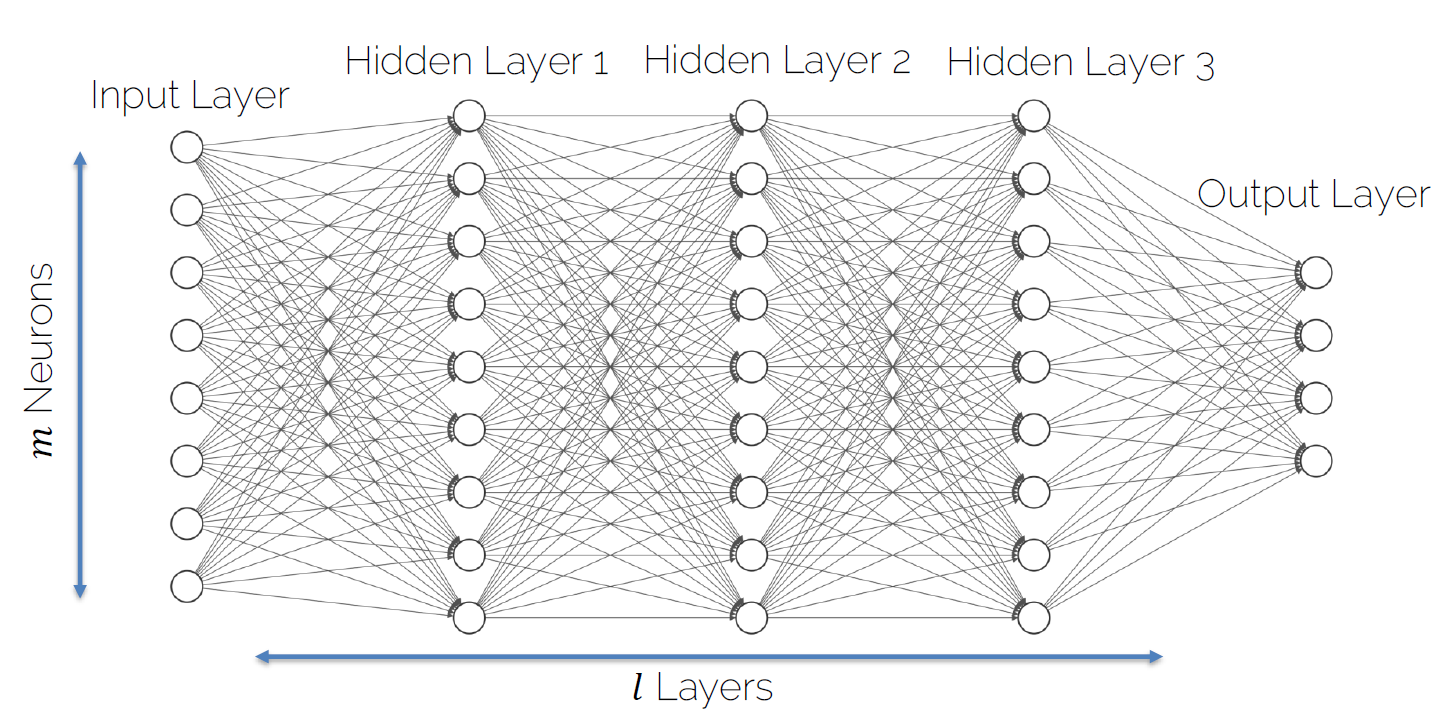
\includegraphics[width=\columnwidth]{figures/nn.png}
\end{figure} ~\\

\textbf{Mathematical Representation}
$$
	L = \mathcal L(y_j, \hat y_j, \theta)
$$
$$
	\hat y_j = a(s_{l,j})
$$
$$
	h_{i,j} = a(s_{i,j})
$$
$$
	s_{i,j} = b_{i,j} + \sum_{k = 1}^m h_{i-1,k} ⋅ w_{i,j,k}
$$
$$
	s_{1,j} = b_{1,j} + \sum_{k = 1}^m x_k ⋅ w_{1,j,k}
$$

\subsection{Number of weights}
\begin{tabular}{ll}	
	$l$: & Depth: number of layers \\
	$m_i$: & Width: number of neurons in layer $i$ (Here: layer $0$ is the input layer)\\
\end{tabular} ~\\

Number of weights is defined as:
$$
	\sum_{i = 1}^l m_i ⋅ m_{i-1} + m_i
$$

\subsection{Forward and Backward Pass}
\subsubsection{Forward Pass/ Forward Propagation}
Use formulas to calculate loss:
$$
	s_{1,1} = b_{1,1} + \sum_{k = 1}^m x_k ⋅ w_{1,1,k} \tab \dots \tab L = \mathcal L(y_j, \hat y_j)
$$

\subsection{Backward Pass/Backward Propagation}
\textbf{Weights of last layer:}
$$
	\frac{\partial L}{\partial w_{l,j,k}} = \frac{\partial L}{\partial \hat y_j} ⋅ \frac{\partial \hat y_j}{\partial s_{l,j}} ⋅ \frac{\partial s_{l,j}}{\partial w_{l,j,k}}
$$

\textbf{Weights of second last layer:}
$$
	\frac{\partial L}{\partial w_{l-1,j,k}} = \sum_{o = 1}^m \frac{\partial L}{\partial \hat y_o} ⋅ \frac{\partial \hat y_o}{\partial s_{l,o}} ⋅ \frac{\partial s_{l,o}}{\partial h_{l-1, j}} ⋅ \frac{\partial h_{l-1, j}}{\partial s_{l-1,j}} ⋅ \frac{\partial s_{l-1,j}}{\partial w_{l-1,j,k}}
$$

\textbf{General:}
$$
	\frac{\partial L}{\partial w_{i,j,k}} = \sum_{o_1 = 1}^m \dots \sum_{o_p = 1}^m \frac{\partial L}{\partial \hat y_{o_1}} ⋅ \frac{\partial \hat y_{o_1}}{\partial s_{l,o_1}} ~~⋅~~ \frac{\partial s_{l,o_1}}{\partial h_{l-1, o_2}} ⋅ \frac{\partial h_{l-1, o_2}}{\partial s_{l-1,o_2}} ⋅ \dots ⋅ \frac{\partial s_{i+1,o_p}}{\partial h_{i, j}} ⋅\frac{\partial h_{i, j}}{\partial s_{i,j}} ⋅ \frac{\partial s_{i,j}}{\partial w_{i,j,k}}
$$

\pagebreak

\section{Training}
\subsection{Learning}
\begin{itemize}
	\item Learning means generalization to unknown dataset, i.e. train on known dataset, test with optimized parameters on unknown dataset
\end{itemize}

\subsection{Dataset}
\begin{itemize}
	\item Split dataset into
	\begin{itemize}
		\item Training data (e.g. 60\%, 80\%) - Used to train the model
		\item Validation data (e.g. 20\%, 10\%) - Validate the current model to find the best hyperparameters
		\item Test data (e.g. 20\%, 10\%) - Is only used once in the end
	\end{itemize}
\end{itemize}

\subsection{Weight initialization}
\textbf{Bad choice:} \\
\begin{itemize}
	\item All weights $= 0$ → No symmetry breaking
	\item Small Random Numbers → Output becomes zero using tanh as activation function → Vanishing gradient
	\item Big Random Numbers → Output saturates to $-1$ and $1$ using tanh as activation function → Vanishing gradient
\end{itemize}

\subsubsection{Xavier Initialization}
\begin{itemize}
	\item Gaussian with zero mean and $var(w) = \frac 1 n$ ($n$: number of weight per neuron)
	\item For ReLU: $Var(w) = \frac 2 n$
\end{itemize}

\subsection{Errors}
\begin{itemize}
	\item Ground truth error
	\begin{itemize}
		\item Faults in dataset, e.g. wrong classification of sample image
		\item Underfitting
	\end{itemize}
	\item Training set error
	\begin{itemize}
		\item Underfitting
	\end{itemize}
	\item Validation/test set error
	\begin{itemize}
		\item Overfitting
	\end{itemize}
\end{itemize}

\subsection{Hyperparameters}
\begin{itemize}
	\item Hyperparameters = Learning Setup + Optimization, i.e.,
	\begin{itemize}
		\item Network architecture (number of layers, number of weights, ...)
		\item Number of iterations
		\item Learning rate(s)
		\item Regularization
		\item Batch size
		\item ...
	\end{itemize}
\end{itemize}

\subsubsection{Hyperparameter Tuning Methods}
\begin{itemize}
	\item Manual search:
	\begin{itemize}
		\item Find out the optimal hyperparameters manually
		\item most common
	\end{itemize}
	\item Grid search:
	\begin{itemize}
		\item Define ranges for all parameters spaces and select points
		\item Iterates over all possible configurations
	\end{itemize}
	\item Random search:
	\begin{itemize}
		\item Like grid search but one picks points at random in the predefined ranges
	\end{itemize}
\end{itemize}

\subsection{Learning Curves}
\subsubsection{Ideal Training}
\begin{itemize}
	\item Small gap between training and validation loss
	\item Training and validation loss go down at the same rate (stable without fluctuations)
\end{itemize}

Example:
\begin{figure}[H]
	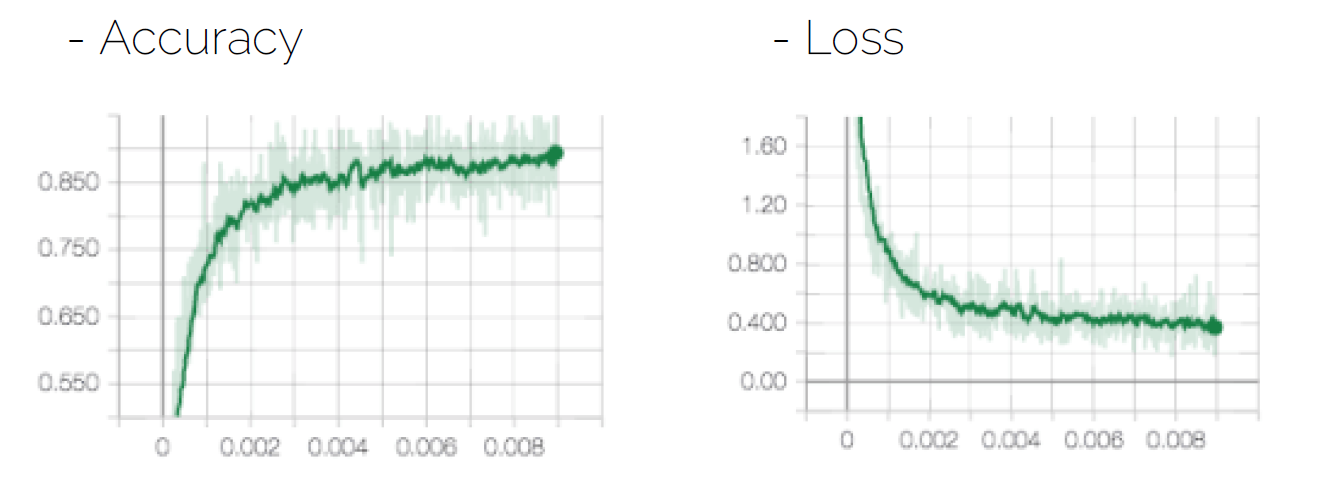
\includegraphics[width=\columnwidth]{figures/l_curves.png}
\end{figure}

\subsubsection{Underfitting}
\begin{itemize}
	\item Training and validation losses decreases even at the end of training
	\item Reasons:
	\begin{itemize}
		\item Model is still learning
	\end{itemize}
\end{itemize}

Example:
\begin{figure}[H]
	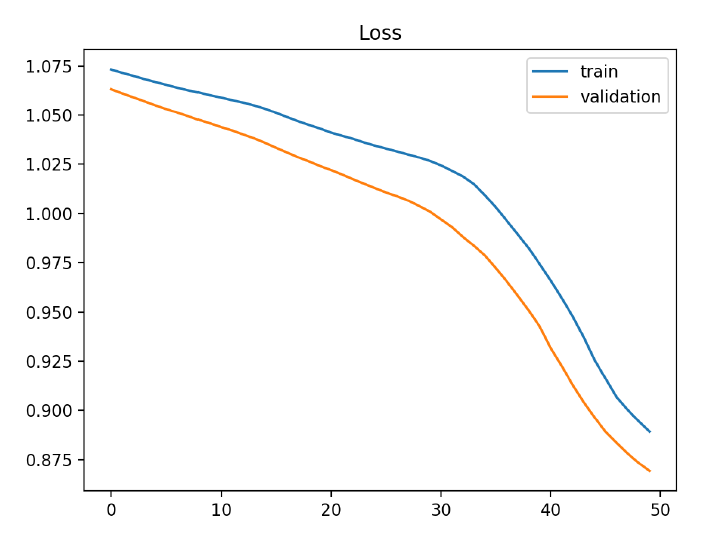
\includegraphics[width=0.5\columnwidth]{figures/graph_underfitting.png}
\end{figure}

\subsubsection{Overfitting}
\begin{itemize}
	\item Training loss decreases and validation loss increases
	\item Reasons:
	\begin{itemize}
		\item Model is memorizing the training samples instead of generalizing
	\end{itemize}
\end{itemize}

Example:
\begin{figure}[H]
	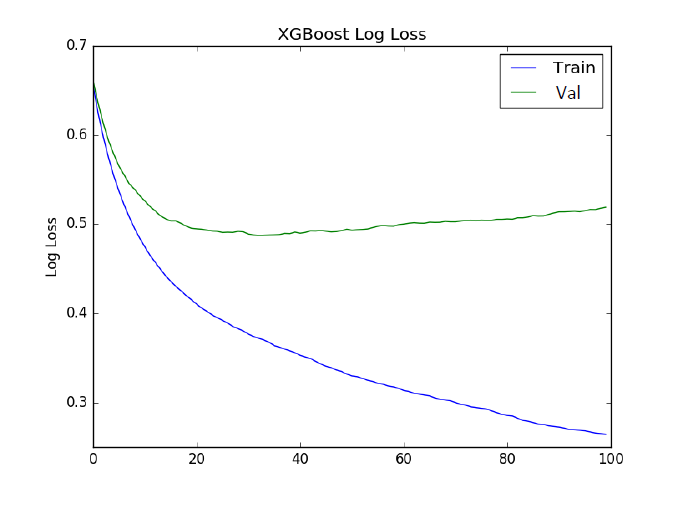
\includegraphics[width=0.5\columnwidth]{figures/graph_overfitting.png}
\end{figure}

\begin{figure}[H]
	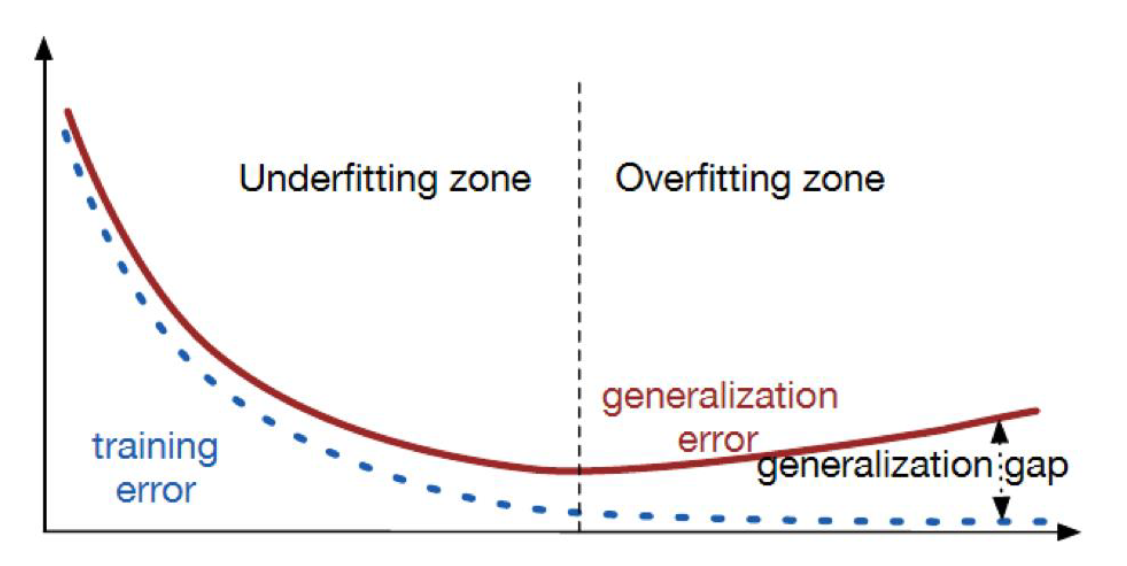
\includegraphics[width=0.7\columnwidth]{figures/graph_underOverfitting.png}
\end{figure}

\subsubsection{Other Examples}
\textbf{Validation set easier than training set:}
\begin{itemize}
	\item Validation loss is lower than training loss
	\item Reasons:
	\begin{itemize}
		\item Validation set is easier than the training set
		\item Bug in the implementation
	\end{itemize}
\end{itemize}

Example:
\begin{figure}[H]
	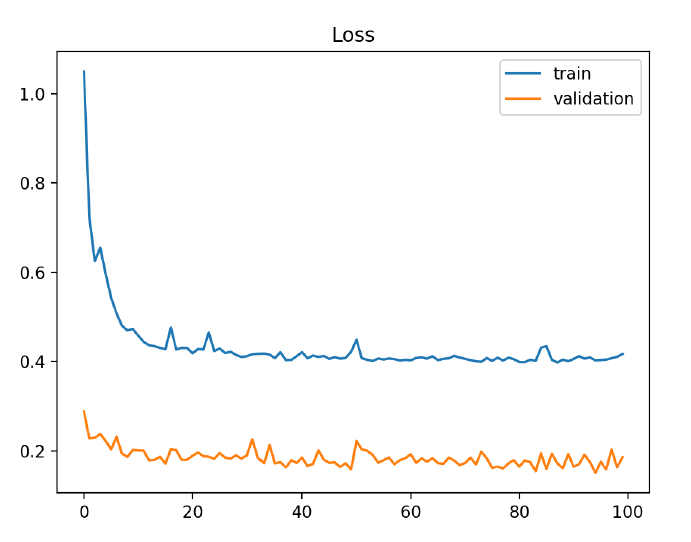
\includegraphics[width=0.5\columnwidth]{figures/graph_val_easy.png}
\end{figure}

\textbf{Learning rate to low:}
\begin{itemize}
	\item Loss curves decrease almost linearly
	\item Reasons:
	\begin{itemize}
		\item The initial Learning rate is too low
	\end{itemize}
\end{itemize}

Example:
\begin{figure}[H]
	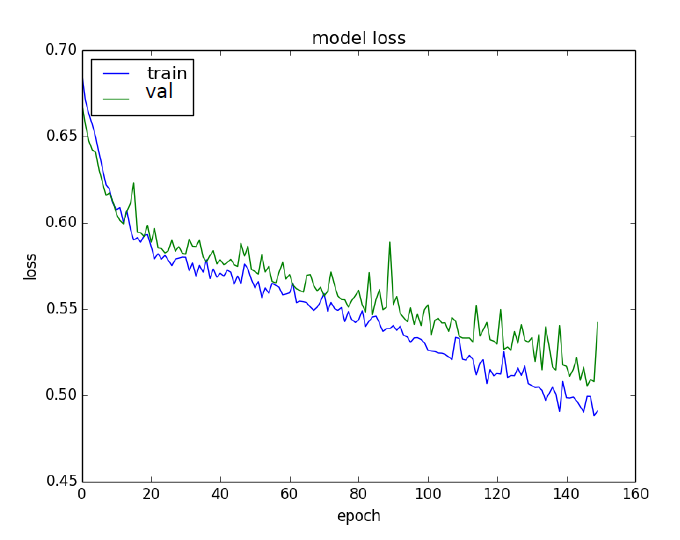
\includegraphics[width=0.5\columnwidth]{figures/graph_lr_low.png}
\end{figure}

\textbf{Learning rate to high:}
\begin{itemize}
	\item Loss curves decrease very quickly at the beginning and then remain on plateaus
	\item Reasons:
	\begin{itemize}
		\item Learning rate is too big
		\item Inconsistent dataset
	\end{itemize}
\end{itemize}

Example:
\begin{figure}[H]
	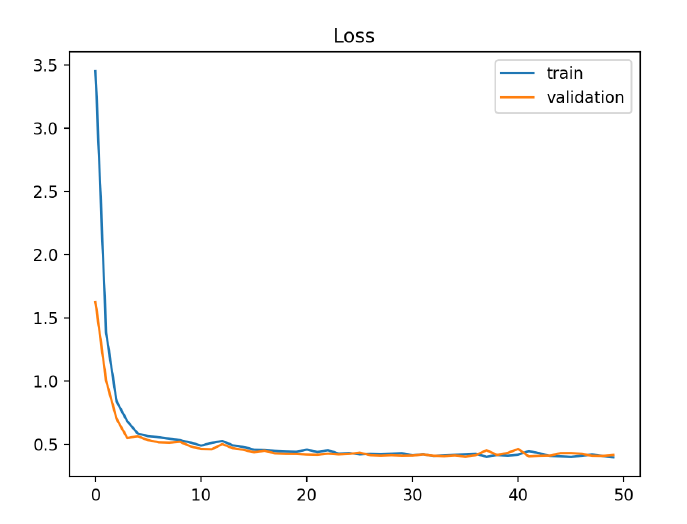
\includegraphics[width=0.5\columnwidth]{figures/graph_lr_high.png}
\end{figure}

\subsection{How To}
\subsubsection{Network Architecture}
\begin{itemize}
	\item Start with the simplest network possible
\end{itemize}
\subsubsection{Training samples}
\begin{enumerate}
	\item Start with a single training sample
	\begin{itemize}
		\item Check if output is correct
		\item Should overfit
		\item Train accuracy should be 100\%
	\end{itemize}
	\item Increase to handful of samples (e.g., 4)
	\begin{itemize}
		\item Check if input is handled correctly
	\end{itemize}
	\item Move to more samples
	\begin{itemize}
		\item 5, 10, 100, 1000, ...
		\item At some point, you should see generalization
	\end{itemize}
\end{enumerate}

\subsubsection{Learning rate}
\begin{itemize}
	\item Find a learning rate that makes the loss drop significantly within 100 iterations
	\item Good learning rates to try: $1e-1, 1e-2, 1e-3, 1e-4$
	\item Good weight decay to try: $1e-4, 1e-5, 0$
	\item Use Grid/Random search
\end{itemize}

\subsubsection{Timings}
\begin{itemize}
	\item Measure how long each iteration takes (should be $< 500 ms$
	\item Look for bottlenecks (e.g. Dataloading, Backpropagation)
	\item Estimate total time
\end{itemize}


\subsubsection{Basic Recipe}
\begin{figure}[H]
	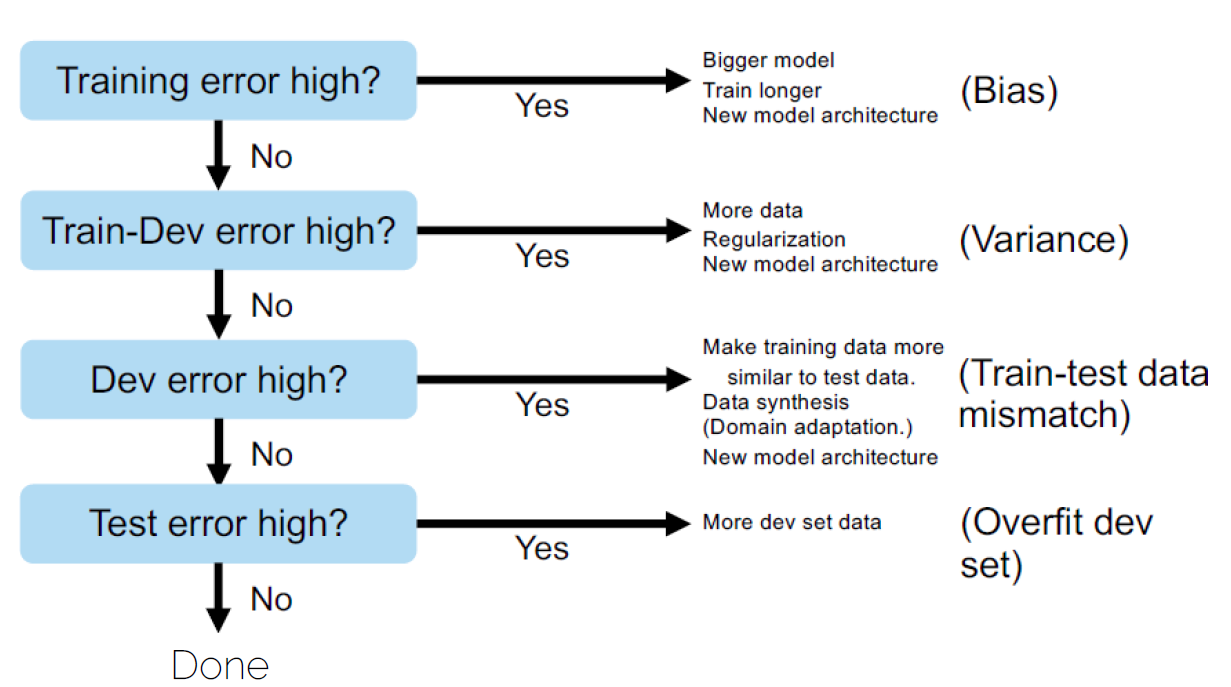
\includegraphics[width=0.7\columnwidth]{figures/recipe.png}
\end{figure}

\subsubsection{Bad Signs}
\begin{itemize}
	\item Training error not going down
	\item Validation error not going down
	\item Performance on validation better than on training set
	\item Tests on train set different than during training
\end{itemize}

\subsubsection{Good/Bad Practice}
\textbf{Good Practice:}
\begin{itemize}
	\item Use train/validation/test curves
	\begin{itemize}
		\item Evaluation needs to be consistent
		\item Numbers need to be comparable
	\end{itemize}
	\item Only make one change at a time
\end{itemize}

\textbf{Bad Practice/Common Mistakes}
\begin{itemize}
	\item Using single batch it did not overfit
	\item Forgot to toggle train/eval mode for network
	\item Forgot to call \lstinline|.zero_grad()| (in PyTorch) before calling \lstinline|.backward()|
	\item Passed softmaxed outputs to a loss function that expects raw logits
	\item Training set contains test data
	\item Debug algorithm on test data
\end{itemize}










\pagebreak
\section*{Notes}
This is a summary of the lecture~\lecture~of the Technical University Munich.
This lecture was presented by~\lecturer~in the~\semseter.
This summary was created by Gaida B.
All provided information is without guarantee.


%\section*{References}
%author. \textit{title}. publisher. location, year, 

\end{document}

%TODO check for todos








